\documentclass{article}
\usepackage[utf8]{inputenc}
\usepackage[margin=0.675in]{geometry}
\usepackage{amsmath}
\usepackage{graphicx}
\usepackage{float}
\usepackage{hyperref}
\usepackage{listings}

\graphicspath{{images/}}
\title{Report for Assignment - Transport Layer - Intranet\\
CS3543 - Computer Networks - 2}
\author{Vishwak Srinivasan\\
\texttt{CS15BTECH11043}}
\date{}

\begin{document}
\maketitle 

\section{Capturing using Intranet Download}
\begin{flushleft}
For this capture, I downloaded the \href{http://intranet.iith.ac.in/files/os/ubuntu-15.04-desktop-amd64.iso}{Ubuntu 15.04 image file}. The duration of the capture was 60 seconds. I used Wireshark on Ubuntu (unlike what was done for Internet Download), since there was LAN and hence no issues with respect to the Network Manager.
\end{flushleft}

\subsection{Plot of Round Trip Time (RTT) versus wall-clock time for 240 seconds}
\begin{flushleft}
This graph was obtained using a graphing tool in Wireshark. You need to go to \texttt{Statistics --> TCP Stream Graphs --> Round Trip Time}, also shown in the picture below:
\begin{figure}[H]
\centering
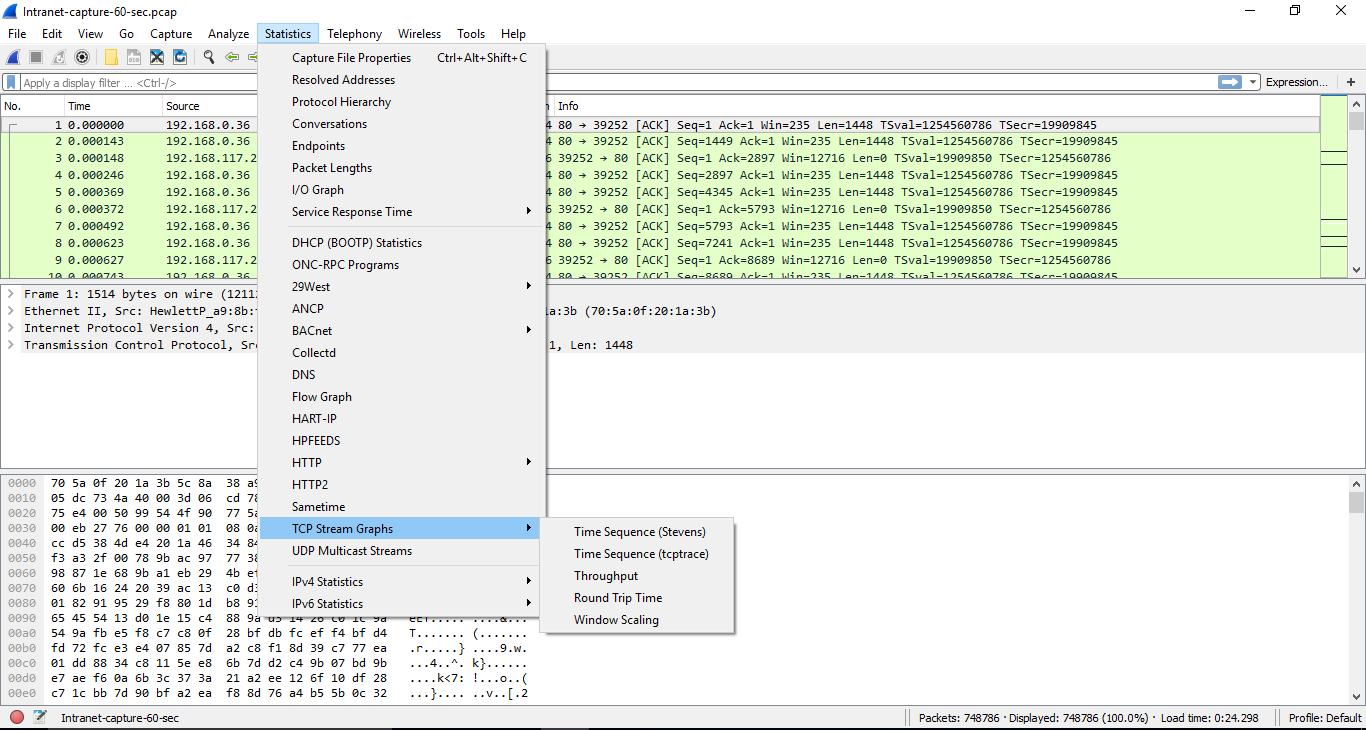
\includegraphics[width=0.6\linewidth]{RTT-Window-size-capture-process-Intranet.png}
\end{figure}

The plot is shown below. The RTT values seem consistent between 0 - 6 milli-seconds, with certain outliers. Observing the \texttt{PCAP} file revealed that these outliers generally occurred in parallel with when the window size was higher.
\begin{figure}[H]
\centering
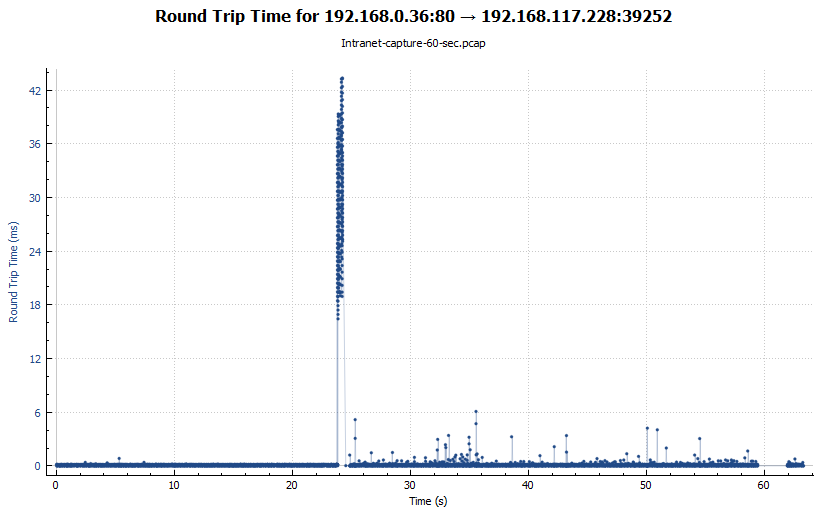
\includegraphics[width=0.65\linewidth]{RTT-variation-60-sec-capture-Ubuntu-time.png}
\end{figure}
\end{flushleft}

\subsection{TCP Congestion Window}
\begin{flushleft}
I have plotted the variation of \texttt{tcp.analysis.bytes\_in\_flight} versus wall-clock time. This provides a reasonable estimate of the TCP congestion window, since this information is actually not advertised.
\begin{figure}[H]
\centering
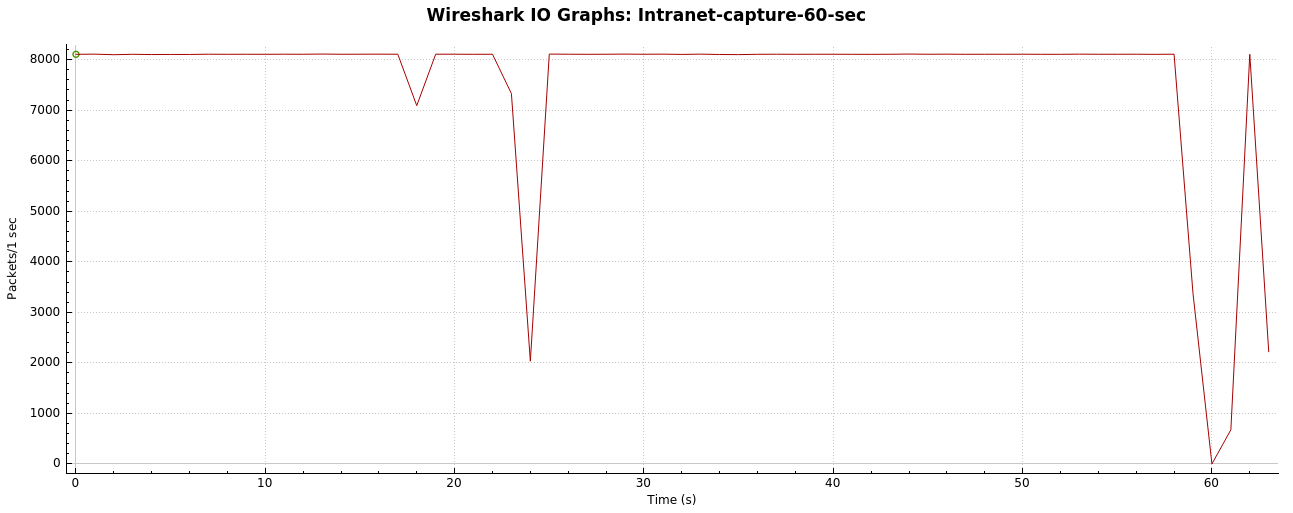
\includegraphics[width=0.75\linewidth]{tcp-CWND-Intranet.png}
\end{figure}
\end{flushleft}

\subsection{Flow Graph}
\begin{flushleft}
Owing the large number of the packets that were captured, the entire flow graph is hard to see in this document, let alone on a 8 GB machine. Below are some snapshots taken despite the lag:
\begin{figure}[H]
\centering
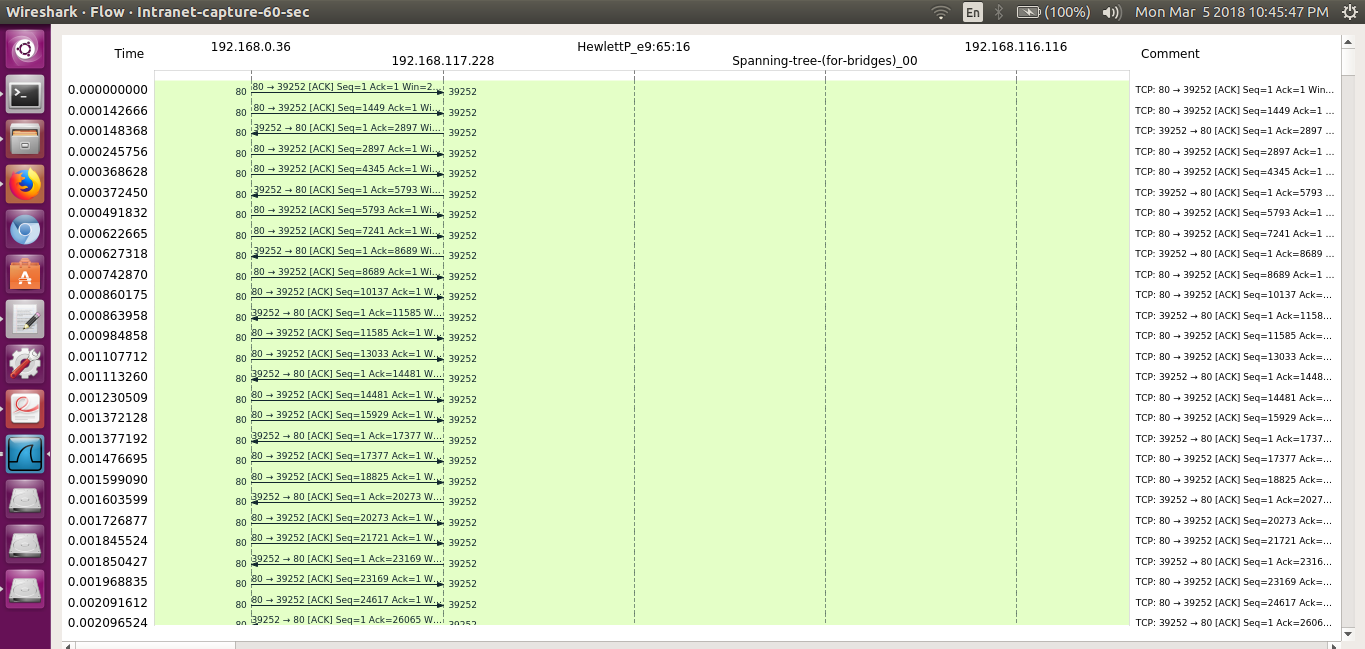
\includegraphics[width=0.6\linewidth]{flow-graph-1-Intranet.png}
\end{figure}
\begin{figure}[H]
\centering
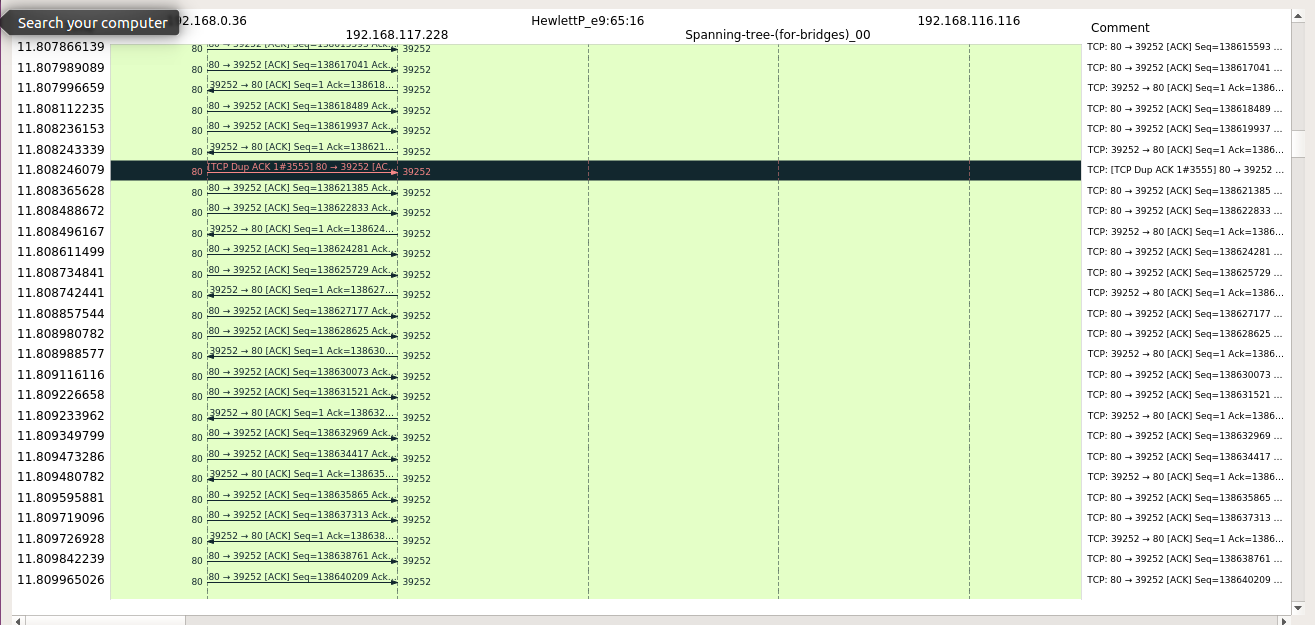
\includegraphics[width=0.6\linewidth]{flow-graph-2-Intranet.png}
\end{figure}
\end{flushleft}

\subsection{Average Throughput and variation of throughput with wall-clock time}
\begin{flushleft}
This graph was again obtained using a graphing tool in Wireshark, available at \texttt{Statistics --> TCP Stream Graphs --> Throughput}. Here the graph is plotted with a moving average over 1 second, and is shown below:
\begin{figure}[H]
\centering
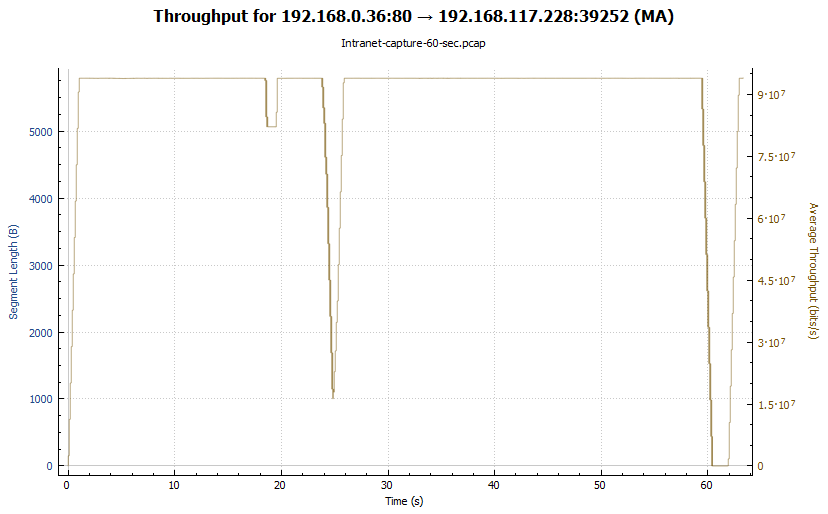
\includegraphics[width=0.55\linewidth]{Throughput-variation-60-sec-capture-Ubuntu.png}
\end{figure}

The average throughput is \(\frac{751694437 \text{ Bytes}}{63.274 \text{ seconds}} \approx \) \boxed{11879989.21 \text{ Bps}} or \boxed{11879.99 \text{ KBps}}. This was obtained through \texttt{Capture File Properties}, and the required image is displayed below:
\begin{figure}[H]
\centering
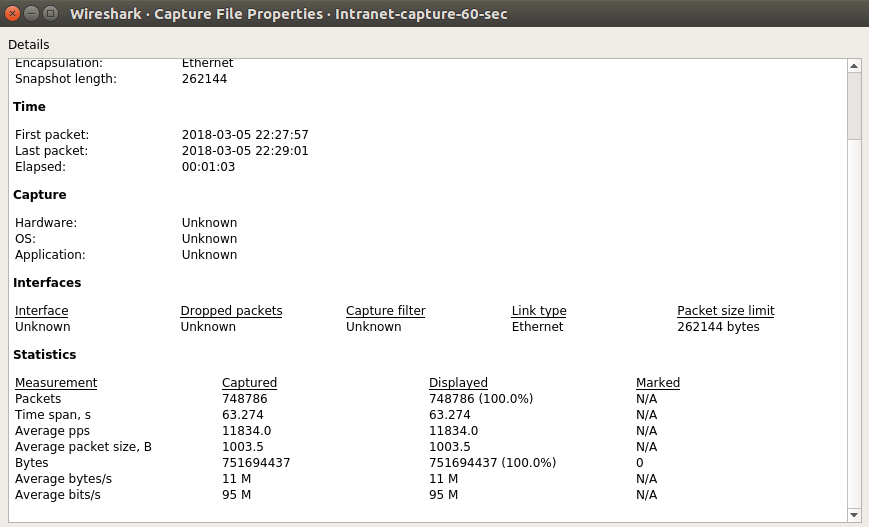
\includegraphics[width=0.55\linewidth]{Packet-capture-stats-60-sec-capture-Ubuntu.png}
\end{figure}
\end{flushleft}

\subsection{Receiver Congestion Window size variation with wall-clock time}
\begin{flushleft}
This graph plots the size of the Congestion Window Size (\texttt{cwnd}), using the same Wireshark graphing tool. Here you can observe that the when window size is higher, the RTT is also higher as shown in the other graph. Eventually, a high window size causes a delay, which is when the window size decreases. This variation is graphically represented below:
\begin{figure}[H]
\centering
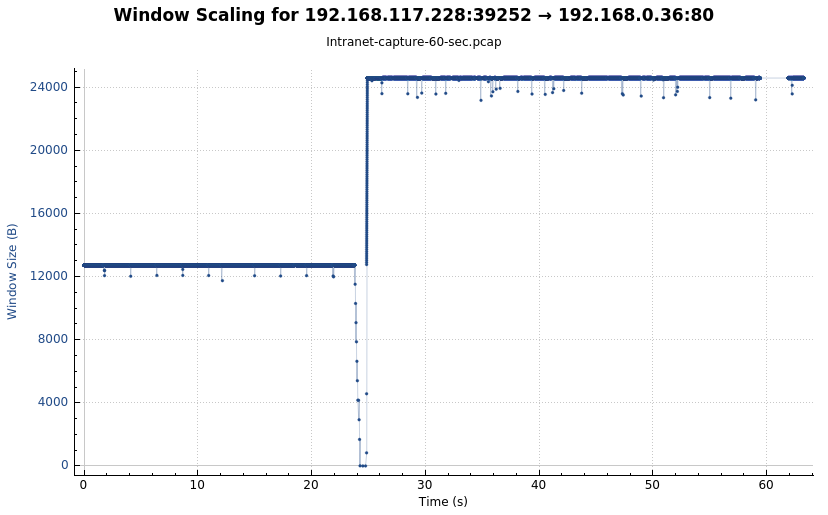
\includegraphics[width=0.55\linewidth]{Window-size-variation-60-sec-capture-Ubuntu.png}
\end{figure}
\end{flushleft}

\subsection{Number of 1-DupACK, 2-DupACK and 3-DupACK with wall-clock time}
\begin{flushleft}
This can be extracted using the filter \texttt{tcp.analysis.duplicate\_ack\_num == <number>}, where \texttt{number} is either 1, 2 or 3 in this case. The filters need to be added to the IO Graph to view the variation graphically, and the process is shown below:
\begin{figure}[H]
\centering
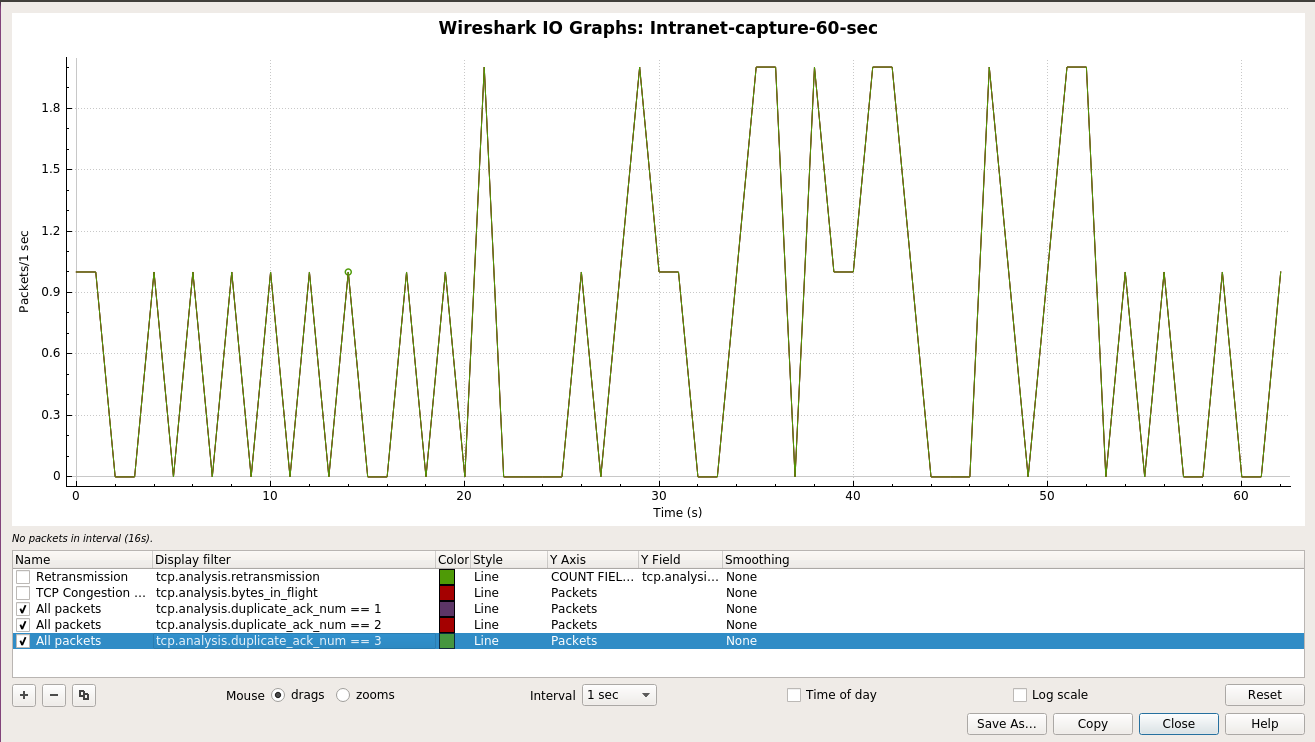
\includegraphics[width=0.55\linewidth]{dup-ack-capture-process-Intranet.png}
\end{figure}

The variation in the number of 1-DupACK, 2-DupACK and 3-DupACK is shown below (top-left: 1-DupACK, top-right: 2-DupACK and bottom-center: 3-DupACK).
\begin{figure}[H]
\begin{minipage}{0.48\linewidth}
\centering
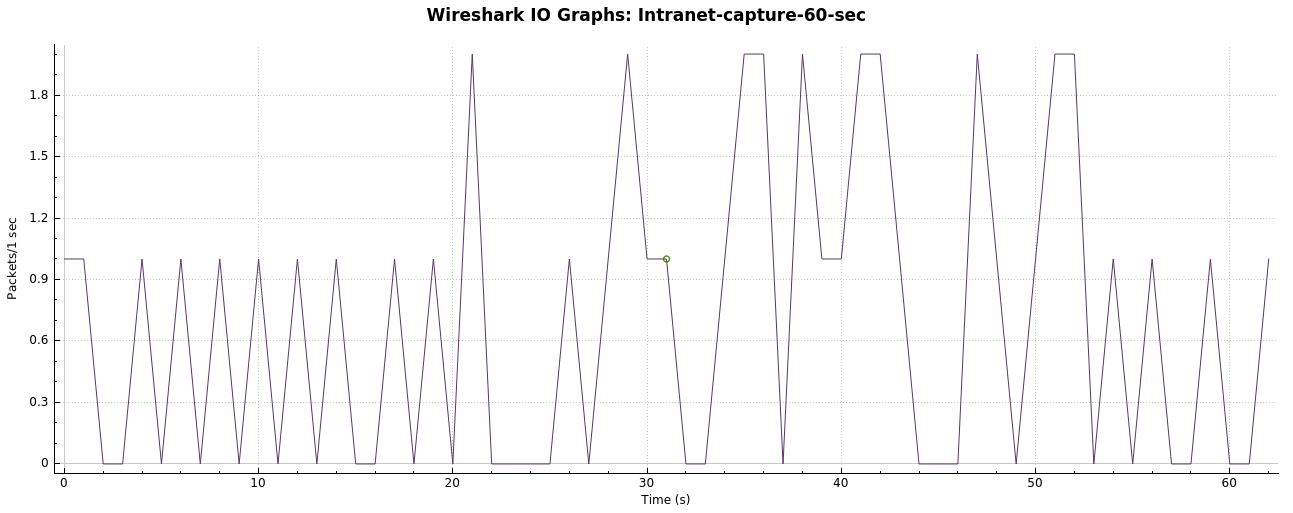
\includegraphics[width=0.975\textwidth]{1-dup-ack-Intranet.png}
\end{minipage}
\hfill
\begin{minipage}{0.48\linewidth}
\centering
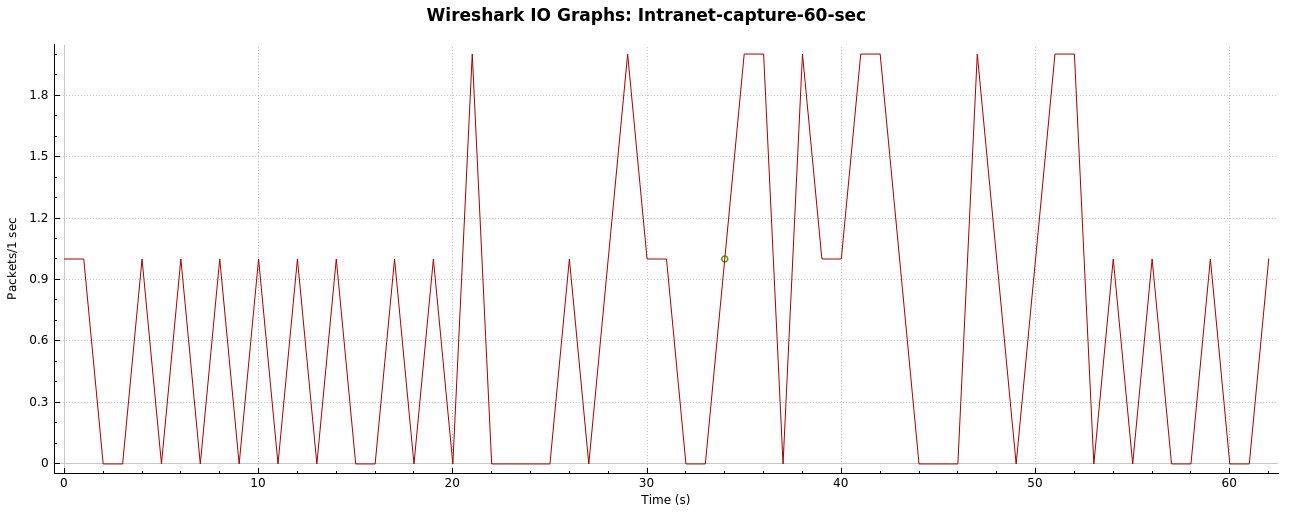
\includegraphics[width=0.975\textwidth]{2-dup-ack-Intranet.png}
\end{minipage}
\end{figure}
\begin{figure}[H]
\centering
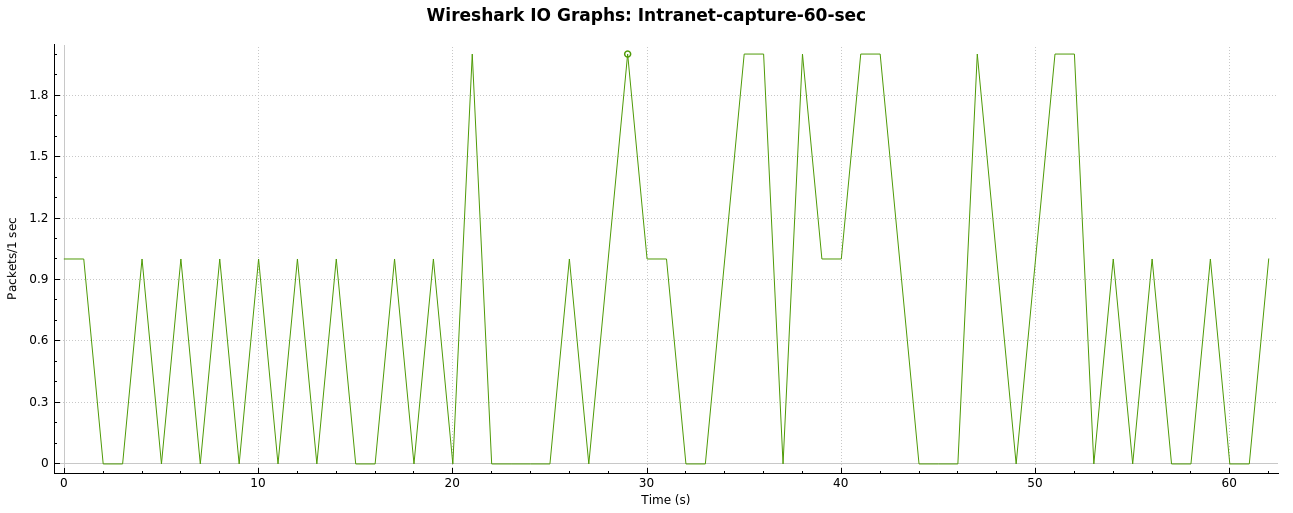
\includegraphics[width=0.47\textwidth]{3-dup-ack-Intranet.png}
\end{figure}
\end{flushleft}
\end{document}
